\begin{figure*}
  \begin{center}
    \begin{tabular}{c}
      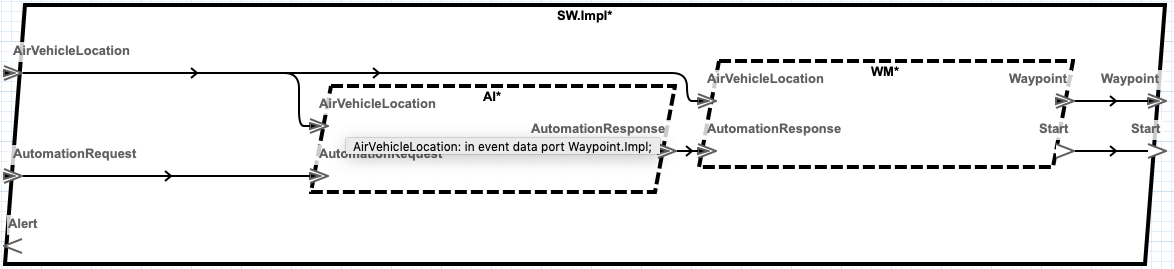
\includegraphics[scale=0.4]{example.png} \\
      (a) \\
      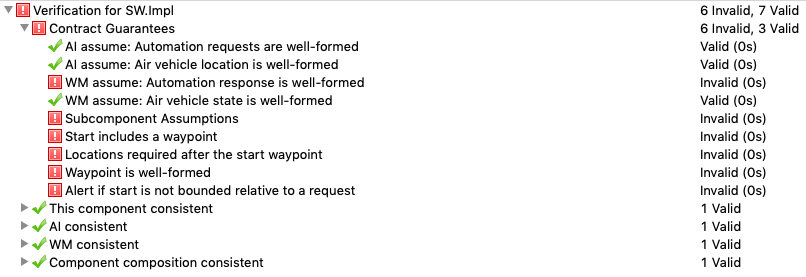
\includegraphics[scale=0.4]{example-certificate.png} \\
      (b)
    \end{tabular}
  \end{center}
\caption{Automated UAV route planning system. (a) Unhardened system. (b) Failure certificate.}
\label{fig:example}
\end{figure*}

\figref{fig:example} is an AADL description of an implementation of a software system for route planning and automated control for a UAV. It is loosely based on the system in the case study presented later. The system receives an automation request that is forwarded to an untrusted third-party route planner (AI) that decides the flight path of the UAV based on its current position and the requested task. The waypoint manager (WM) receives the mission command as a set of waypoints from the planner and starts the UAV flying the mission, issuing waypoints to the UAV flight controller as the UAV location changes. It is an \emph{as is} legacy component. The alert manager never raises the alert as there is no capacity in the design to know when an alert is needed.

The goal is to cyber-harden the system so that it is resilient to cyber-attack. For this simple example, two attacks are considered; both attacks originating from the untrusted route-planner: first, malformed messages to disrupt the waypoint manager or UAV flight control; and second, a delayed or unrequested automation response to prevent the UAV from flying a mission or to fly the wrong mission.

\newsavebox{\sw}
\begin{lrbox}{\sw}
\begin{lstlisting}[style=agree]
eq req : bool = event(AutomationRequest);
eq avl : bool = event(AirVehicleLocation);
eq wp : bool = event(Waypoint);
eq rsp: bool = event(Start);
eq alrt : bool = event(Alert);
            
assume "Automation request is well-formed" :
    req => WELL_FORMED_AUTOMATION_REQUEST(AutomationRequest);
assume "Air vehicle location is well-formed" :
    avl => WELL_FORMED_WAYPOINT(AirVehicleLocation);
    
eq nothing : bool = (not req) -> (not pre (req)) and (not req);
eq today : bool = req and rsp;    
eq yesterday : bool = false -> pre (req and not rsp);
eq policy : bool = nothing
                or (today and not yesterday)
                or (not today and rsp and yesterday);
eq since : bool = (alrt and (false -> pre(since))) 
               or (not policy and alrt);

guarantee "Start includes a waypoint" :
    rsp => wp;
guarantee "Locations required after the start waypoint" :
    (wp and not rsp) => avl;
guarantee "Waypoint is well-formed" :
    wp => WELL_FORMED_WAYPOINT(Waypoint);
guarantee "Alert if start is not bounded relative to a request" :
    (policy and not alrt) or since;
\end{lstlisting}
\end{lrbox}

\begin{figure}
  \begin{center}
    \scalebox{0.60}{\usebox{\sw}}
  \end{center}
  \caption{The SW component contract.}
  \label{fig:sw}
\end{figure}

This work uses an assume guarantee paradigm, in the form of contracts, to model and hierarchically prove properties of the system (cite AGREE). The contracts constrain the inputs and state properties of output for component models. In this example, the model for the route planner assumes its input is well-formed, but it makes no guarantees about its output as it is an untrusted third party component. The contract for the legacy waypoint manager makes similar assumptions about its input, but unlike the route planner, the model constrains its output to be well-formed and coincide with the mission command from the route planner and the air vehicle location.\footnote{See \cite{repo} for the full model.}

The contract to model the SW component with its primary inputs and outputs is in \figref{fig:sw}. The contract language is a first order predicate calculus. The contract semantics are synchronous data-flow where the inputs, outputs, and expressions are characterized by data streams. The semantics are such that the contracts are evaluated in dependency order with inputs being propagated to outputs through all the contracts until they stabilize; as such, the contracts, and thereby the system model, must be acyclic. Once the contracts have stabilized, then the model takes a synchronous step to the next input data in the stream. The semantics do not model computation or communication delay. The output of one contract is seen at the input of any downstream contract in the same step of the input data stream. 

The contract in \figref{fig:sw} uses \texttt{eq} statements to define variables local to the contract. For example, the \texttt{req} variable is equivalent to the \texttt{event(req)} expression. An \texttt{event} expression is true if there is data on the named AADL event port. The system contract assumes well-formed input and guarantees a set of properties about the output.

There are two requirements in the SW model, among others, related to the cyber-attacks: the first, \emph{Waypoint is well-formed} disallows malformed waypoints from being propagated; and the second, \emph{Alert if start is not bounded relative to a request}, disallows a mission being started without a request or if the start is delayed more than one step after a request. This later guarantee merits some further discussion as it illustrates the steam nature of the semantics.

The guarantee is an invariant on the expression \texttt{(policy and not alrt) or since} meaning that either the policy holds and there is no alert or the alert has been sounding since the policy was first violated. The \texttt{policy} is satisfied if there is no pending request (\texttt{nothing}), a request with a response right now (\texttt{today}), or a request yesterday with its response today. The value of \texttt{nothing} and \texttt{yesterday} in the current time step rely on values from the previous time step. The \texttt{yesterday} uses the \texttt{->} operator for initialization. The left operand is the initial value of \texttt{yesterday} at the start of the system, which in this example is \texttt{false} because there is no yesterday at the start.  The right operand is the value of \texttt{yesterday} after the initial step. Here the \texttt{pre} operator refers to the value of \texttt{(req and not rsp)} in the prior time step. Intuitively, \texttt{yesterday} is true if the previous time step made a request without a matching response. 

The value of \texttt{since} relies on its own value in the previous time step. The intuitive reading of the expression is that the alert has been true since the time when the policy first failed. The first failure sets \texttt{since} to true (i.e., \texttt{(not policy and alrt)}), and once \texttt{since} true, it persists as long as \texttt{alrt} holds. As such, the \emph{Alert if start is not bounded relative to a request} guarantee defines one behavior of a correctly implemented system. In this way, the contracts model the expected input and output of the system as a whole, and they also model the expected behavior of each component used to implement the system.

Model checking proves whether the contract models of the components, with their connections, implement the system model in \figref{fig:sw}. The results of the model checker are in \figref{fig:example}(b). Not unexpectedly, since the model of the route planner leaves the output behavior unconstrained (i.e., the component can do anything since it is not trusted) the model checker proves that the component composition does not implement the system requirements.

\begin{figure*}
  \begin{center}
    \begin{tabular}{c}
      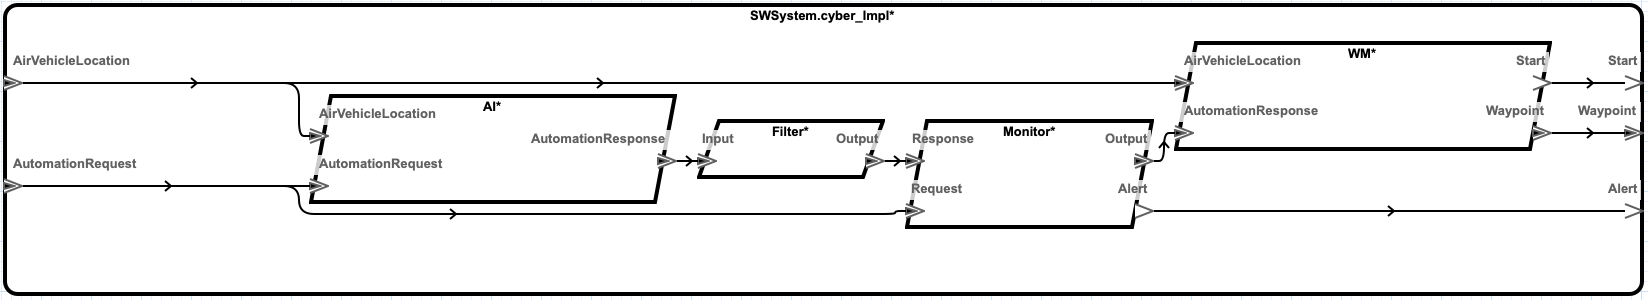
\includegraphics[scale=0.3]{hardened.png} \\
      (a) \\
      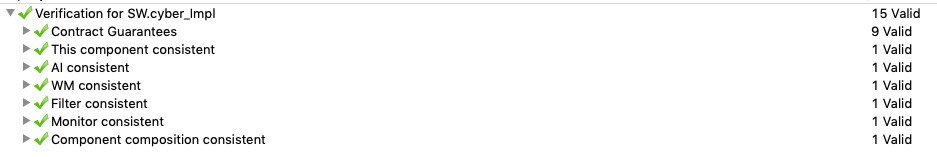
\includegraphics[scale=0.4]{hardened-certificate.png} \\
      (b)
    \end{tabular}
  \end{center}
  \caption{Hardened UAV system. (a) The implementation with high-assurance components. (b) Passing certificate.}
  \label{fig:hardened}
\end{figure*}

\newsavebox{\flt}
\begin{lrbox}{\flt}
\begin{lstlisting}[style=agree]
eq policy : bool = 
  WELL_FORMED_AUTOMATION_RESPONSE(Input);       
guarantee Filter_Output "Filter output is well-formed" :
  if event(Input) and policy then 
    event(Output) and Output = Input
  else not event(Output);
\end{lstlisting}
\end{lrbox}

\newsavebox{\mntr}
\begin{lrbox}{\mntr}
\begin{lstlisting}[style=agree]
const is_latched : bool = 
Get_Property(this, CASE_Properties::Monitor_Latched);
eq rsp : bool = event(Response);
eq req : bool = event(Request);
eq nothing : bool = (not req) -> (not pre (req)) and (not req);
eq today : bool = req and rsp;    
eq yesterday : bool = false -> pre (req and not rsp);
eq policy: bool = nothing
               or (today and not yesterday)
               or (not today and rsp and yesterday);
eq alert : bool = (not policy) 
               -> ((is_latched and pre(alert)) or not policy);
guarantee Monitor_Alert 
  "Alert port tracks alert variable" :
  event(Alert) = alert;
guarantee Monitor_Output
  "Output if not alerted" :
  if event(Alert) then (not event(Output)) else
  if event(Response) then (event(Output) and (Output = Response))
  else (not event(Output));
\end{lstlisting}
\end{lrbox}

\begin{figure}
  \begin{center}
    \begin{tabular}{c}
      \scalebox{0.60}{\usebox{\flt}} \\
      (a) \\
      \scalebox{0.60}{\usebox{\mntr}} \\
      (b)
    \end{tabular}
  \end{center}
  \caption{High-assurance component contracts. (a) The filter. (b) The monitor.}
  \label{fig:assurance}
\end{figure}

The system implementation is cyber-hardened by using the CASE tools to insert high-assurance components in the form of a filter and a monitor as shown in \figref{fig:hardened}(a). A filter enforces an invariant over each datum in the data stream by not forwarding input to its output if that input is violating. Its stylized form as generated by the tool is shown in \figref{fig:assurance}(a). The user must declare the meaning of the \texttt{policy} value as part of the transform on the model. In this example, \texttt{policy} is the assumption made by the waypoint manager about the automation response being well-formed. The output guarantees are automatically generated by the tool.

A monitor captures a relation over time on input data and is able to reason about temporal properties of that input. By definition, it raises an alert output when the relation is violated. The generated monitor contract is shown in \figref{fig:assurance}(b). The \texttt{is\_latched} value makes the alert persistent meaning that once raised always raised. The definition for \texttt{policy} is taken from the contract in \figref{fig:sw} since this high-assurance component is the monitor that needs to alert violations of the bounded response policy. As before the guarantees for the outputs are autogenerated by the tool.

The proof certificate for the new cyber-hardened implementation is in \figref{fig:hardened}(b). The high-assurance components guarantee the correct behavior of the SW implementation in the presence of the considered cyber attacks.

\newsavebox{\cml}
\begin{lrbox}{\cml}
\begin{lstlisting}[style=myML]
fun filter_step () =
let val () = Utils.clear_buf buffer
    val () = API.callFFI "get_input" "" buffer
    val string = Utils.buf2string buffer
in
    if WELL_FORMED_AUTOMATION_RESPONSE string
    then
        let val string = Word8Array.substring buffer 1
                         (Word8Array.length buffer - 1)
        in API.callFFI "put_output" string Utils.emptybuf
        end
    else print"Filter rejects message.\n"
end
\end{lstlisting}
\end{lrbox}

\begin{figure}
  \begin{center}
    \begin{tabular}{c}
      \scalebox{0.60}{\usebox{\cml}}
    \end{tabular}
  \end{center}
  \caption{Synthesized CakeML for the filter.}
  \label{fig:cakeml}
\end{figure}

The high-assurance components are automatically synthesized from the contract models to equivalent models in the CakeML language. The synthesized CakeML code for the filter is shown in \figref{fig:cakeml}. The code is called at dispatch by the scheduler. The \texttt{API.callFFI} is the link to the communication fabric to capture input and provide output. The body of the function restates the filter contract to make the appropriate assignments in a way that matches the truth value of the predicate in the filter guarantee.

CakeML itself provides a complete verified compilation to binaries for several different platforms meaning that the resulting binaries exactly preserve the meaning of the original CakeML code. A similar proof is given for the synthesis of the contract model for a high-assurance component to CakeML. A high-assurance component contract has a precise meaning in terms of data streams, and the synthesis exactly preserves that meaning in the resulting CakeML. In other words, for any set of input streams that meet the component's contract assumptions, the output streams from the synthesized CakeML exactly match the output streams from the high-assurance component's contract. 

Preserving the input/output relationship of streams between the two models lifts the contract verification results to the deployed system. If the contract model verifies, then the meaning of those results hold for the deployed system if the other components implement their contracts, an appropriate schedule exists that follows the dependent data-flow, and the communication fabric works as expected.
